% !TeX TXS-program:compile = txs:///pythonlualatex

\documentclass[a4paper,11pt]{article}
\usepackage[revgoku]{cp-base}
\graphicspath{{./graphics/}}
%variables
\donnees[%
	classe={1\up{ère} 2M2},matiere={[SPÉ.MATHS]},mois=Février,annee=2022,typedoc=CHAP,numdoc=7
	]
%formatage
\author{Pierquet}
\title{\nomfichier}
\hypersetup{pdfauthor={Pierquet},pdftitle={\nomfichier},allbordercolors=white,pdfstartview=FitH,pdfborder=0 0 0}
%divers
\lhead{\entete{\matiere}}
\chead{\entete{\lycee}}
\rhead{\entete{\classe{} - \mois{} \annee}}
\lfoot{\pied{\matiere}}
\cfoot{\logolycee{}}
\rfoot{\pied{\numeropagetot}}

\begin{document}

\pagestyle{fancy}

\part{CH07 - Dérivation locale - Exercices (Correction)}

\smallskip

\exonum{0}

\begin{enumerate}
	\item On obtient $f(3)=\dfrac{3+1}{2-3}=\dfrac{4}{-1}=-4$ et la calculatrice donne $f'(3)=3$.
	\item Une équation de $T_3$ est $y=f'(3) \times (x-3) + f(3) = 3(x-3)+(-4)=3x-9-4=3x-13$.
\end{enumerate}

\begin{center}
	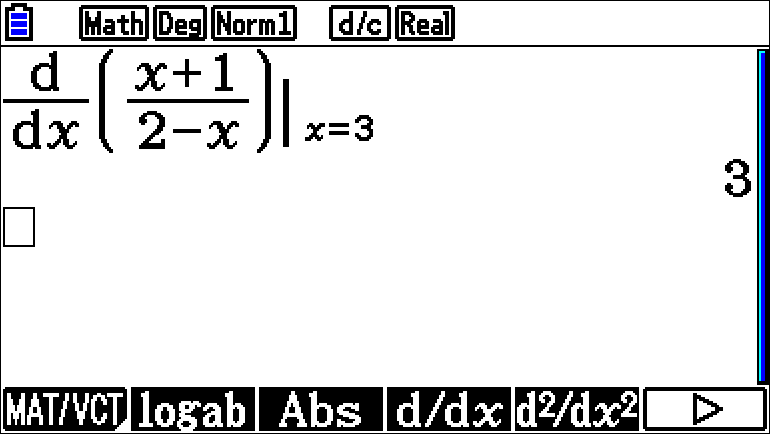
\includegraphics[height=3cm]{chap07_exos_corr_1}
\end{center}

\medskip

\exonum{1}

\begin{enumerate}
	\item  On a $g(1)=\dfrac{2}{1^2+1}=\dfrac{2}{2}=1$.
	\item On a $\lim_{h \to 0} \dfrac{g(1+h)-g(1)}{h} = \lim_{h \to 0}\dfrac{-h-2}{h^2+2h+2} = \dfrac{-2}{2}=-1$.
	
	Ceci justifie que $g$ est dérivable en $a=1$ et que $g'(1)=-1$.
	\item Une équation de $T_1$ est $y=g'(1) \times (x-1) + g(1) = -1(x-1)+1 = -x+2$.
\end{enumerate}

\begin{center}
	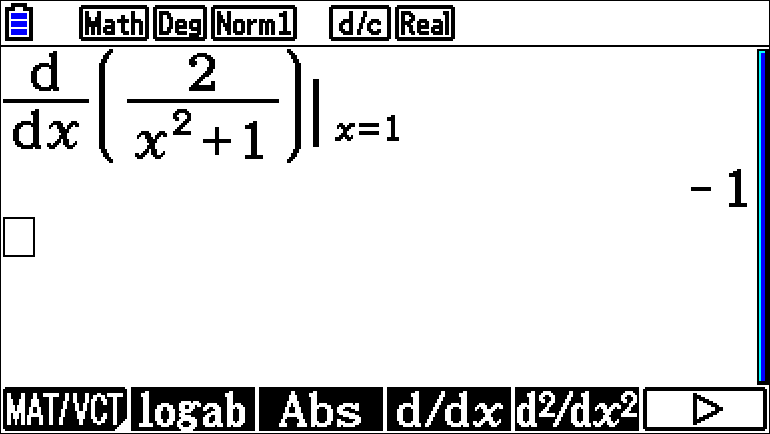
\includegraphics[height=3cm]{chap07_exos_corr_2}
\end{center}

\medskip

\exonum{2}

\begin{enumerate}
	\item La fonction $h$ semble être dérivable en toute valeur de $\intervFF{-3}{9}$ car la courbe $\mathscr{C}_h$ est \og bien lisse \fg{}.
	
	Il n'y a pas de \og cassure verticale \fg, de \og verticalité \fg{} ou de \og point anguleux \fg.
	\item On rappelle que $h(\ldots)$ correspond à la \textit{hauteur de la courbe}, et $h'(\ldots)$ à la pente de la tangente :
	\begin{enumerate}
		\item $h(4)=-1,5$ et $h'(4)=\text{pente de }T_4=\dfrac{3}{4}$ ;
		\item $h(1)=-2$ et $h'(1)=\text{pente de }T_1=0$ ;
		\item $h'(-2)$ est (strictement) négatif, car $T_2$ est décroissante.
	\end{enumerate}
	\item Une équation de $T_1$ est $y=h'(1) \times (x-1) + h(1) = 0(x-1) + (-2) = -2$ (horizontale !).
	
	Une équation de $T_4$ est $T_4 = h'(4) \times (x-4) + h(4) = 0,75(x-4)+(-1,5) = 0,75x-3-1,5=0,75x-4,5$.
	\item[Bonus] $h'(x) \pg 0$ signifie que $h$ est croissante, donc $h'(x) \pg 0$ pour $x \in \intervFF{1}{7}$.
\end{enumerate}

\newpage

\exonum{4}

\medskip

Cet exercice correspond à l'\textsf{activité d'introduction} du \textbf{chapitre 8}, sur les fonctions dérivées.

\medskip

\exonum{5}

\medskip

\begin{pyconcode}
def f(x):
	return x**2

def g(x):
	return 1/x

def mystere(fonc,a,h):
	return (fonc(a+h)-fonc(a))/h

\end{pyconcode}

\begin{enumerate}
	\item 
	\begin{enumerate}
		\item La commande \cpy{mystere(f,2,0.0001)} va calculer $\dfrac{f(2+h)-f(2)}{h}$ pour $f(x)=x^2$ et pour $h = 0,0001$.
		
		On cherche donc à \og estimer \fg{} $\lim_{h \to 0} \dfrac{f(2+h)-f(2)}{h}$ soit encore $f'(2)$, qui vaut (environ) $4$.
		\item La commande \cpy{mystere(f,2,0.0001)} va calculer $\dfrac{g(-5+h)-g(-5)}{h}$ pour $g(x)=\dfrac{1}{x}$ et pour  $h = 0,0001$.
		
		On cherche donc à \og estimer \fg{} $\lim_{h \to 0} \dfrac{g(-5+h)-g(-5)}{h}$ soit encore $g'(-5)$, qui vaut (environ) $-0,04=\tfrac{-1}{25}$.
	\end{enumerate}
	\begin{envconsolepython}[15cm]
		mystere(f,2,0.0001)
		mystere(g,-5,0.0001)
	\end{envconsolepython}
	\item 
	\begin{enumerate}
		\item Pour se référer à l'exercice l'\textcolor{titrebleu}{exercice 2}, on doit déclarer la fonction $g(x)=\dfrac{2}{x^2}$ en \cpy{return 2/(x**2+1)}.
		\item La commande \cpy{mystere(g,1,0.0001)} donnerait un résultat proche de $g'(1) = -1$.
	\end{enumerate}
	\begin{envconsolepython}[15cm]
		def g(x):
			return 2/(x**2+1)
		
		mystere(g,1,0.0001)
	\end{envconsolepython}
\end{enumerate}

\begin{center}
	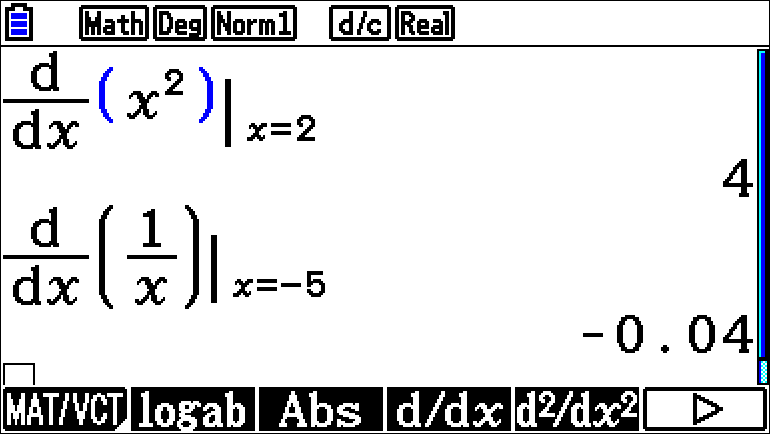
\includegraphics[height=3cm]{chap07_exos_corr_5}
\end{center}

\end{document}